\subsection{Yagi Antenna Fun: How Long is the Driven Element?}

\begin{tcolorbox}[colback=gray!10, colframe=black, title=E9D05] Approximately how long is a Yagi’s driven element?
\begin{enumerate}[label=\Alph*.]
    \item 234 divided by frequency in MHz
    \item 1005 divided by frequency in MHz
    \item 1/4 wavelength
    \item \textbf{1/2 wavelength}
\end{enumerate} \end{tcolorbox}

\subsubsection{Related Concepts}

To understand the question of how long a Yagi’s driven element is, we need to delve into basic antenna theory and the principles of wavelength in radio frequency communications. A Yagi-Uda antenna, commonly known as a Yagi antenna, consists of a driven element, reflector, and directors. The driven element is responsible for receiving or transmitting the radio signal.

The length of the driven element is typically designed to be a specific fraction of the wavelength corresponding to the frequency of operation. For most cases, especially bistatic Yagi antennas, the driven element is designed to be approximately half of the wavelength of the frequency being utilized.

\subsubsection{Calculating Wavelength}

The wavelength (\(\lambda\)) can be calculated with the formula:

\[
\lambda = \frac{c}{f}
\]

where:
- \(c\) is the speed of light in vacuum (\(3 \times 10^8 \text{ m/s}\))
- \(f\) is the frequency in Hertz (Hz)

Since frequencies are typically expressed in Megahertz (MHz) in radio communications, we convert MHz to Hz:

\[
1 \text{ MHz} = 10^6 \text{ Hz}
\]

Thus, the formula in terms of MHz becomes:

\[
\lambda \text{ (in meters)} = \frac{300}{f \text{ (in MHz)}}
\]

For the Yagi’s driven element, which is half of this wavelength, we have:

\[
\text{Length of the driven element} = \frac{1}{2} \times \lambda = \frac{150}{f \text{ (in MHz)}}
\]

This concept aligns closely with choice D, which is equivalent to saying that the driven element is approximately half the wavelength.

\subsubsection{Conclusion}

Understanding the relationship between frequency, wavelength, and antenna structure is crucial for anyone involved in radio communications. A Yagi’s driven element, being half a wavelength, reflects how antenna design optimizes performance based on the operating frequency. This understanding underscores the importance of choosing the right frequency for effective communication.

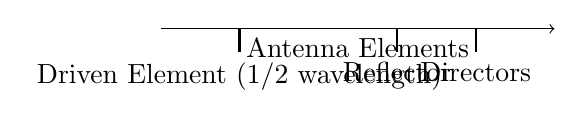
\begin{tikzpicture}
\draw[->] (0,0) -- (5,0) node[midway, below] {Antenna Elements};
\draw[thick] (1,0) -- (1,-0.3) node[below] {Driven Element (1/2 wavelength)};
\draw[thick] (3,0) -- (3,-0.3) node[below] {Reflector};
\draw[thick] (4,0) -- (4,-0.3) node[below] {Directors};
\end{tikzpicture}
